\documentclass[twocolumn,aps,prb,citeautoscript]{revtex4-1}
\input{../preamble_paper.tex}

\begin{document}

\newcolumntype{R}[1]{>{\raggedleft\arraybackslash}p{#1}}

\title{Progress Report 1: Magnetic field profile of a third-scale model for the nEDM experiment}
\author{A. Biswas}
\affiliation{Kellogg Radiation Laboratory, California Institute of Technology}

\maketitle

\section{Motivation}

Charge-parity (CP) violation plays a critical role in explaining matter-antimatter asymmetry
and guiding theories beyond the Standard Model.
The experimental search for instances of CP violation is ongoing \cite{cpv,ill}.
A nonzero electric dipole moment (EDM) in the neutron would constitute such a violation and can be measured
through the shift in Larmor precession frequency of
ultra-cold neutrons (UCN) in $\vec E$ and $\vec B$ fields \cite{pendlebury}.
An upper limit of $2.9 \times 10^{-26}\;e\cdot\text{cm}$ was established in 2006\cite{ill}.

Experiments using these methods 
are prone to a geometric phase (GP) effect, caused by gradients of the magnetic
field, that can lead to a false signal.
\cite{ill,pendlebury} Eliminating the GP effect requires precise engineering
to create a space-uniform magnetic field. Field uniformity also elongates the spin polarization
relaxation time $T_2$ \cite{coil}, allowing more measurement time before the signal deteriorates.

We are constructing a third-scale model of a shielded magnet
to create a field suitable for a more precise nEDM measurement.
New structural features of the third-scale are based on studies of a previous
half-scale model and simulations of superconducting shielding geometries.\cite{rotshield} 

Precise measurements of the magnetic field profile in this new model are needed to determine the potential
effectiveness of its components in the full-scale nEDM experiment, which will take place at Oak Ridge
National Laboratory (ORNL). Field gradients near the shielding and near
the center of the magnet are particularly good indicators of how well the
superconducting shielding can enforce field uniformity and mitigate the GP effect.

\section{Construction of the $\boldsymbol{B_0}$ coil}

At the center of the third-scale model is the $B_0$ coil, a cylindrical structure designed to generate
an uniform field in its interior. A wire is wound around the surface of the cylindrical
plastic frame at locations
that correspond to a $\cos\theta$ coil geometry \cite{coil}, creating a field in the $\xhat$ direction.
The frame used for the winding is adapted from the previous half-scale model.

The third-scale will use superconducting wire, but copper wire was used for test windings
and initial field maps. To distribute tension, the wire is wound around pegs supported by springs
which remain under compression during the winding. The compression stages of the first two windings revealed
structural weaknesses in the new frame. Supports were added to distribute pressure along the circumference. Figure
\ref{winding} shows the first successful test winding of the third-scale $B_0$ coil.

\begin{figure}
\includegraphics[width=\linewidth]{pics/winding.jpg}
\caption{\label{winding}Winding the $B_0$ coil with copper wire.}
\end{figure}

\section{Mapping the $\boldsymbol{B_0}$ coil}

The $B_0$ coil was placed in a cylindrical ferromagnetic shield made out of a Metglas magnetic alloy. The
Metglas promotes $\vec B$ field lines perpendicular to its surface, reinforcing field uniformity by directing
field lines along the $\xhat$ direction. A direct current is supplied to the $B_0$ coil.

We simulate this configuration in \texttt{RotationShield}, a C++ program developed previously in the group
\cite{rotshield} to calculate $\vec B$ fields for environments with cylindrical symmetry. The code finds the 
Green's function and convolves it with the boundary conditions of the Metglas shield and other magnetic components.

In the lab, the $\vec B$ field is mapped with a 3-axis magnetic probe controlled by a stepper motor. Various systematic
errors in this data are corrected in a data analysis program\cite{plotter} which I developed during my 2014 SURF.
One important source of error is the miscentering of the magnetic probe. The stepper motor's origin
is some displacement $\vec{\Delta r} = (\Delta x, \Delta y, \Delta z)$ away from the true magnetic origin. Symmetric
measurements of the field allow us to reset the motor's origin and minimize $\vec{\Delta r}$, but not to
the precision we require.

The simulated field at a position, $\hat{\vec B}(\vec r)$, should be compared with the measured field at the
offset-corrected location, $\vec B(\vec r - \vec{\Delta r})$. In our previous analysis, components of $\vec{\Delta r}$,
most importantly $\Delta x$, were adjusted by hand until the simulated and measured fields agreed along a
small region of interest. A major drawback is that this process is a function of the region of interest.
Furthermore, due to the smaller size of the third-scale model, this offset $\vec{\Delta r}$ has a larger effect on
the field than before.

An automated process including the entire field is preferable. We treat the offset $\vec{\Delta r}$ as
an adjustable parameter and find the deviation of the field from the simulation:
\begin{align*}
\chi^2 (\vec{\Delta r}) &= \sum_{\text{points}}
{|\vec B(\vec r) - \hat{\vec B}(\vec r +\vec{\Delta r})|^2
\over
|\vecr{\sigma}(\vec r)|^2,
}
\end{align*}
where $\vecr{\sigma}(\vec r)$ is the uncertainty in the measurement of $\vec B(\vec r)$ and the summation
is taken over all measured field points in a volume.

Since \texttt{RotationShield} gives discrete output, interpolation of the simulated field $\hat{\vec B}$
is required for this routine. A Markov chain Monte Carlo (MCMC) algorithm will be used to
vary $\vec{\Delta r}$ until $\chi^2(\vec{\Delta r})$ is minimized. An efficient implementation of this routine
is under construction.

\section{Thermal Shielding Problem}

One of the main magnetic shielding components is superconducting lead. The third-scale
model inherits a cylindrical lead shield as well as lead endcaps from its half-scale predecessor. The model
is placed in a cryostat to cool the lead below $T_c = 7\un{K}$ and enter the superconducting phase.
To map the field, our regions of interest (near magnetic center) must be in a warm bore, thermally shielded
from the cryostat.

This thermal shield includes a layer of copper. In an alternating magnetic field,
large-scale eddy currents would be induced in the copper plating and affect the magnetic field. To avoid this,
we use a layer of copper strands attached with epoxy. The strands are insulated
and currents cannot jump between them, ideally preventing the creation of large-scale eddy currents.

To test the effectiveness of the copper-strand thermal shield (henceforth simply the thermal shield),
we apply an alternating current to the $B_0$ coil creating a field:
\begin{align*}
\vec B = \xhat B_0 \cos(\omega t + \psi).
\end{align*}
The amplitude $B_0$ and phase $\psi$ are measured with the magnetic probe
and an oscilloscope relative to a reference signal at the same frequency $\omega$.
A square copper plate is placed such that the magnetic probe is on the plate's central axis, resulting in a
disturbed field:
\begin{align*}
\vec{B'} = \xhat B_0' \cos(\omega t + \psi').
\end{align*}
The disturbed amplitude and phase $B_0'$ and $\psi'$ are measured relative to the same reference signal,
and the gain $\gamma$ and phase shift $\Delta\psi$ are recorded:
\begin{align*}
\text{gain: }\gamma \equiv {B_0' \over B_0}, \sp{} \text{phase shift: } \Delta\psi \equiv \psi' - \psi.
\end{align*}
The experiment is repeated with a square of our thermal shielding.

Figures \ref{gain} and \ref{phase} show measurements of
$\gamma(\omega)$ and $\Delta\psi(\omega)$ for the thermal shield and the copper plate. Analysis of this
data is ongoing, and an analytical solution for $\gamma(\omega)$ and $\Delta\psi(\omega)$ incorporating skin
depth shielding and induced fields is being developed.


\begin{figure*}
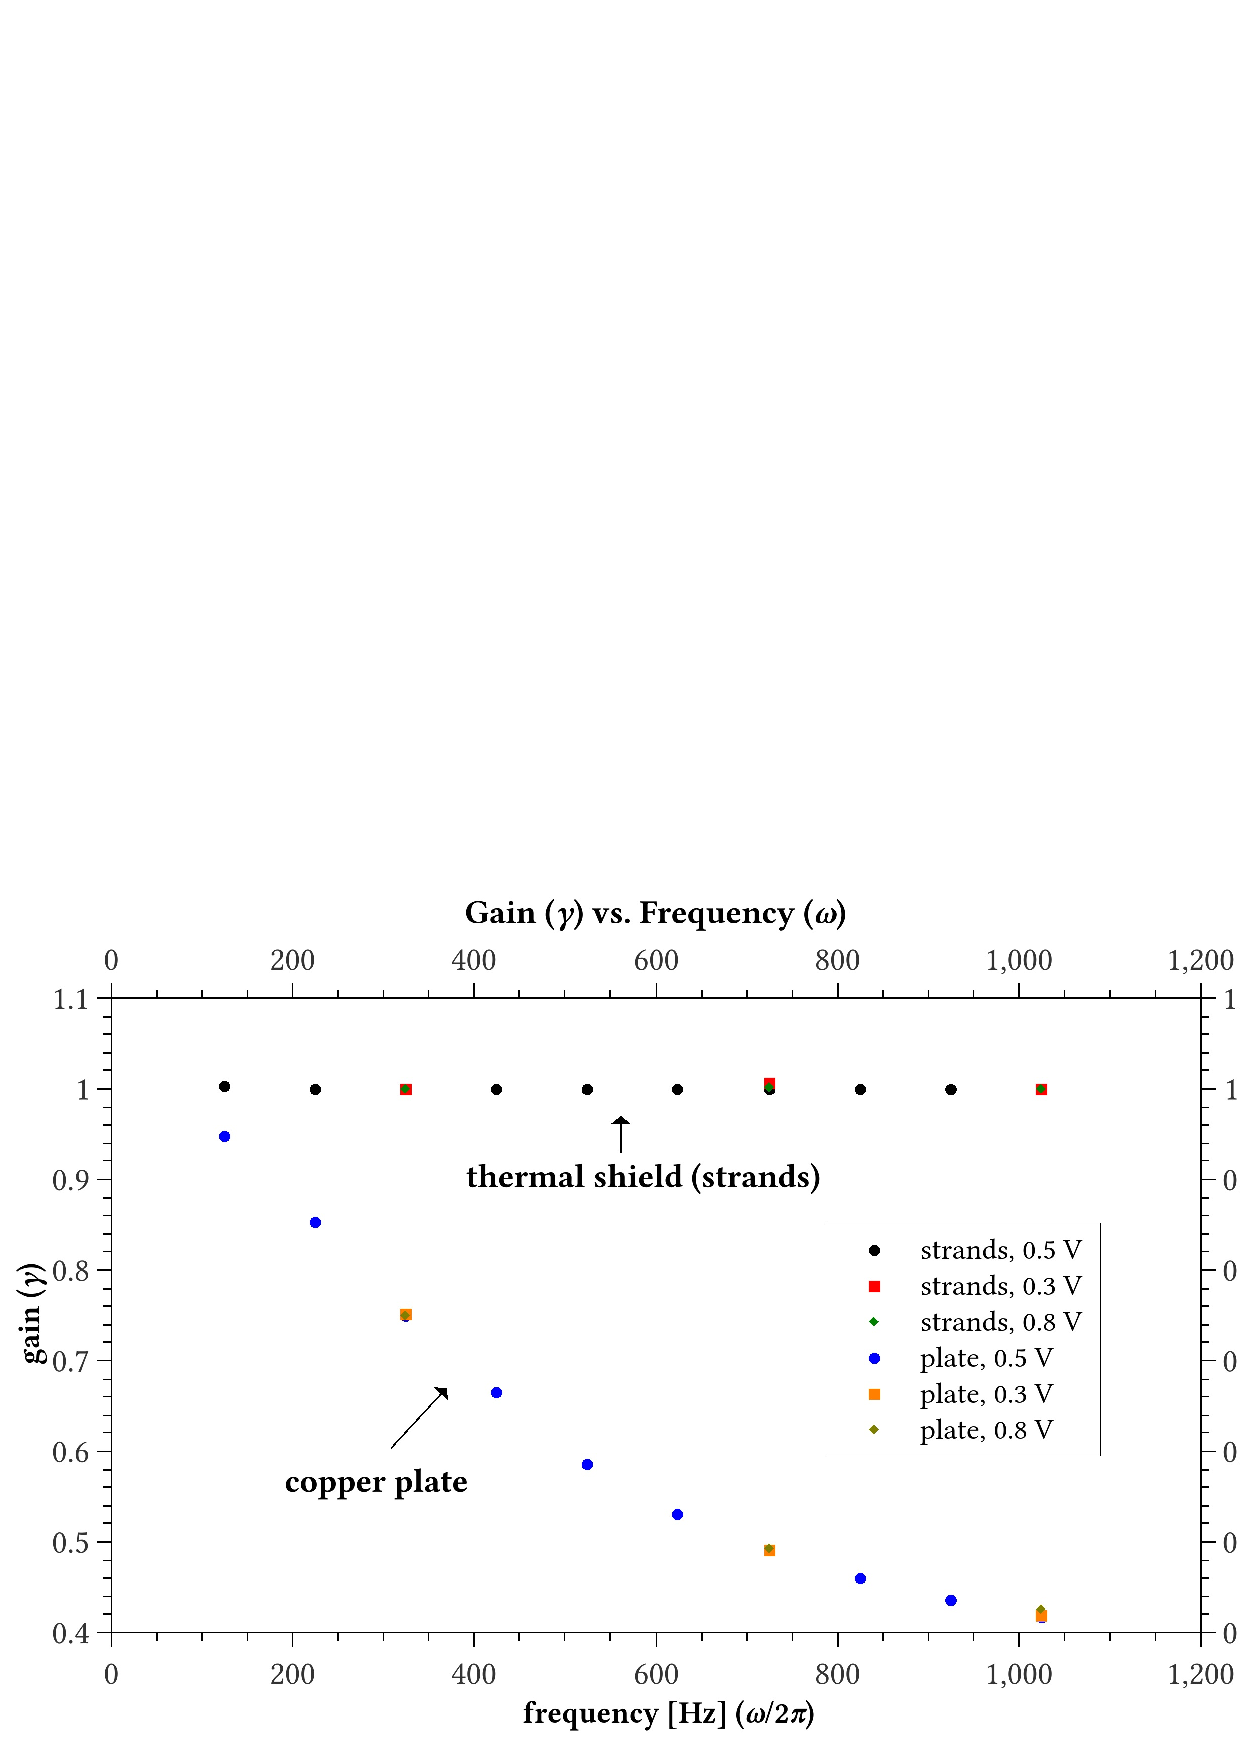
\includegraphics[width=0.9\linewidth]{savedplots/Graph1.pdf}
\caption{\label{gain} Gain $\gamma = B_0' / B_0$ of the disturbed field (in the presence of copper) relative
to the undisturbed field.}
\end{figure*}
\begin{figure*}
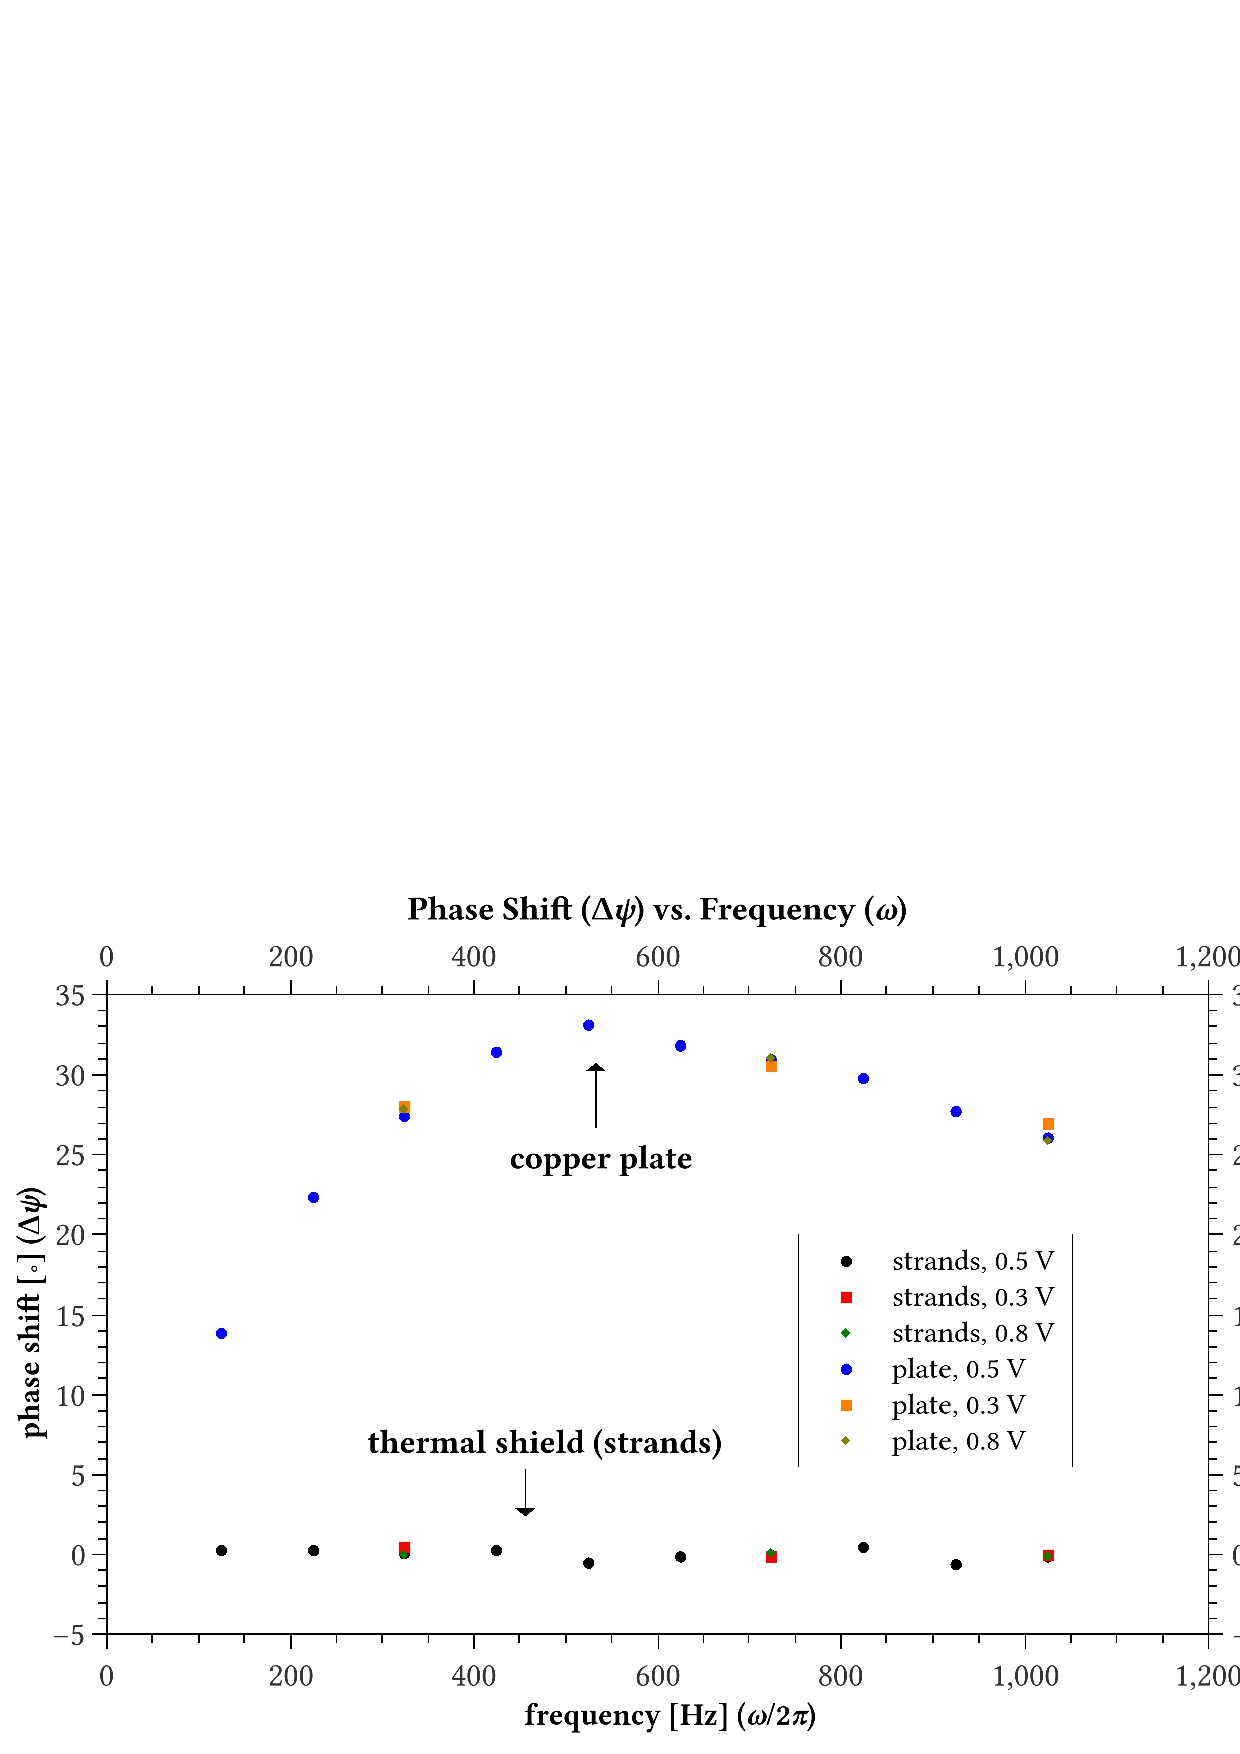
\includegraphics[width=0.9\linewidth]{savedplots/Graph2.pdf}
\caption{\label{phase} Phase shift $\Delta\psi = \psi' - \psi$
of the disturbed field (in the presence of copper) relative to the undisturbed field.}
\end{figure*}

\begin{thebibliography}{}
\bibitem{cpv} J. Cronin, ``Nobel Lecture: CP Symmetry'' (2013).
\bibitem{ill} C.A. Baker, et al., Phys. Rev. Lett. 97 (2006) 131801.
\bibitem{pendlebury} J.M. Pendlebury et al., Phys. Rev. A 70 (2004) 032102.
\bibitem{endcapstyles} S. Malkowski, IEEE Trans. Magn. 49 (2013) 651.
\bibitem{coil} A. Perez Galvan et al., Nucl. Instrum. Meth. A 660 (2011) 147.
\bibitem{rotshield} M.P. Mendenhall, $\langle$github.com/mpmendenhall/rotationshield$\rangle$.
\bibitem{plotter} A. Biswas, $\langle$github.com/xerebus/nedm$\rangle$.
\end{thebibliography}

\end{document}
